\subsection{Time savings and sensitivity analyses}
\label{subsec:noah__snr}

\begin{figure}[htb]
    \centering
    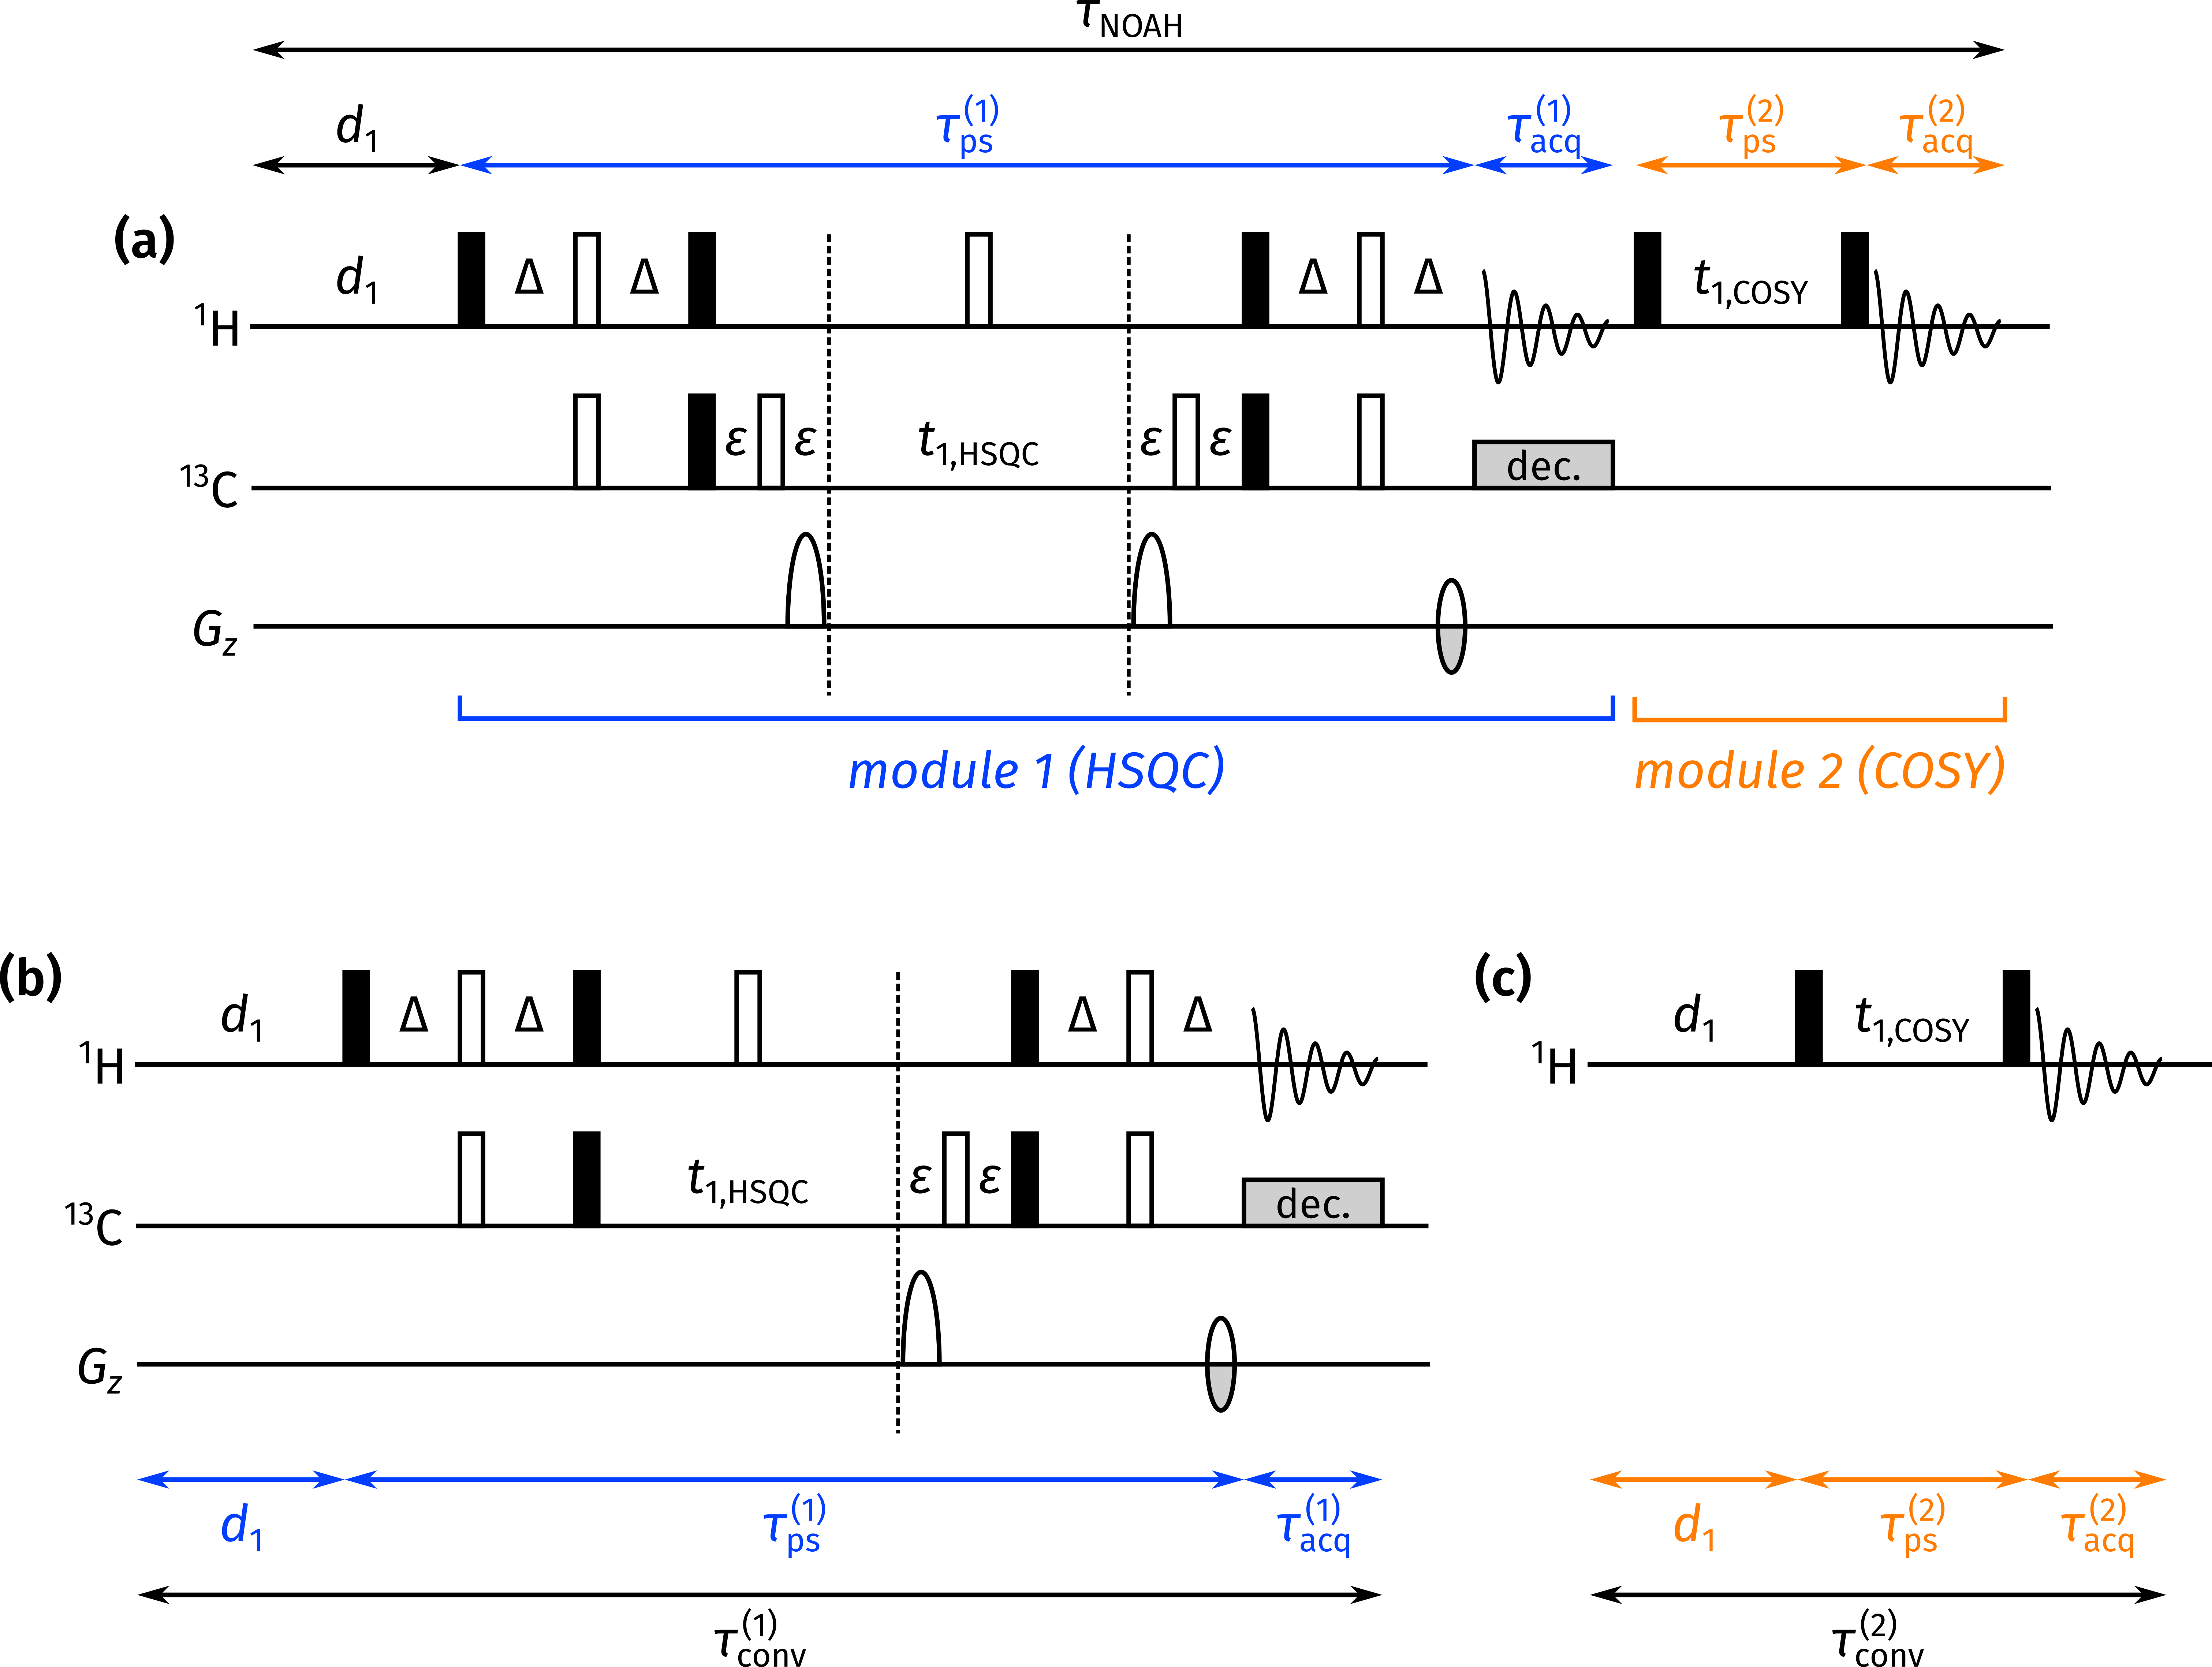
\includegraphics[]{noah/timings.png}%
    {\phantomsubcaption\label{fig:noah_timings_noah_sc}}%
    {\phantomsubcaption\label{fig:noah_timings_conv_s}}%
    {\phantomsubcaption\label{fig:noah_timings_conv_c}}%
    \caption[Comparison of NOAH and conventional 2D experiments]{
        \textbf{(\subref*{fig:noah_timings_noah_sc})} \noah{S,C} supersequence, comprising HSQC and COSY modules (see \cref{tbl:noah_modules} for an explanation of the single-letter module codes used).
        \textbf{(\subref*{fig:noah_timings_conv_s})} `Conventional' echo--antiecho HSQC (the same as in \cref{fig:hsqc_etgp}).
        \textbf{(\subref*{fig:noah_timings_conv_c})} `Conventional' COSY.
        The timings referred to in the text are highlighted for all three experiments; I have assumed that $d_1$ for each experiment is the same.
        Note that the lengths are not to scale: $d_1$ is typically far longer than the $\tau_\text{ps}$ and $\tau_\text{acq}$.
    }
    \label{fig:noah_timings}
\end{figure}

In a typical 2D NMR experiment, the majority of the experiment duration is taken up by the \textit{recovery delay}---the time required for spins to return to their equilibrium polarisation, such that the next transient or $t_1$ increment can be recorded.
The removal (or shortening) of recovery delays is thus a very effective way of speeding up 2D data acquisition.
In NOAH supersequences, 2D experiments (`modules') can be directly concatenated without the addition of extra recovery delays between them: only one overall recovery delay is required for the entire supersequence.
This means that, to a first approximation, a supersequence containing $N$ modules ($N \geq 2$) can be acquired in the time needed for just one module.
\Cref{fig:noah_timings} shows an example of a NOAH supersequence formed from two modules (HSQC and COSY): the various timings referred to in the text which follows are also marked on the diagram.

The duration of an NMR experiment, $\tau_\text{exp}$, can be expressed as a sum of its parts:
\begin{equation}
    \label{eq:exp_duration_2d}
    \tau_\text{exp} = \tau_\text{ps} + \tau_\text{acq} + d_1,
\end{equation}
where $\tau_\text{ps}$ is the time required for the pulse sequence itself (typically several milliseconds), $\tau_\text{acq}$ is the acquisition time (several hundred milliseconds), and $d_1$ is the recovery delay (one or more seconds).
The \textit{time-saving factor} $\rho_t$ for a NOAH supersequence, as compared to a series of conventional standalone experiments, is then:
\begin{equation}
    \label{eq:rho_t}
    \rho_t
    = \frac{\sum_i \tau_\text{conv}^{(i)}}{\tau_\text{NOAH}}
    = \frac{{\sum_i (\tau_\text{ps}^{(i)} + \tau_\text{acq}^{(i)} + d_1^{(i)})}}{d_1 + \sum_i (\tau_\text{ps}^{(i)} + \tau_\text{acq}^{(i)})},
\end{equation}
where $\tau_\text{NOAH}$ is the duration of the NOAH experiment, $\tau_\text{conv}$ is the duration of a conventional experiment, and the superscript $(i)$ represents the $i$-th module or conventional experiment being acquired.
The sum runs from $i = 1$ to $N$, where $N$ is the number of modules.
If we assume that $d_1^{(i)} = d_1$ is the same for all $N$ conventional experiments and the supersequence, then in the limit where
\begin{equation}
    \label{eq:d1_limit}
    d_1 \gg \sum_i \tau_\text{ps}^{(i)} + \tau_\text{acq}^{(i)},
\end{equation}
we have that $\rho_t \to Nd_1/d_1 = N$.
This analysis makes plenty of assumptions, and is not entirely valid in practice.
For example, \textit{each} $\tau_\text{acq}$ is often around 5\text{--}10\% of $d_1$, so is not entirely negligible, especially in longer supersequences.
Furthermore, some modules require longer $\tau_\text{ps}$: most notable is the NOESY module, which contains a mixing time of several hundred milliseconds. (HMBC, TOCSY, and ROESY spectra are also lesser offenders.)
These factors serve to reduce $\rho_t$ from its idealised value of $N$; generally, this deviation is larger as $N$ increases, because \cref{eq:d1_limit} becomes less and less valid.
Nevertheless, the general point that time savings are approximately proportional to $N$ stands.

For relatively concentrated samples, where sensitivity is not an issue, we can in fact end the discussion here.
In this \textit{sampling-limited regime}, the minimum 2D experiment duration is dictated purely by the number of $t_1$ increments needed to obtain sufficient resolution in the indirect dimension, as well as the minimum phase cycle required for artefact suppression.%
\footnote{With modern gradient-enhanced experiments, the minimum phase cycle may well not even be a `cycle'; see also \cref{fig:hsqc_comparison}.}
NOAH supersequences are identical to conventional experiments in both aspects, but provide a time-saving factor of $\rho_t \sim N$.

The development of modern NMR instrumentation, including high-field magnets and cryogenic probes, means that the sampling-limited regime continues to be extended to ever lower concentrations.
However, it is often not this simple: the opposite \textit{sensitivity-limited regime} is still very commonly encountered, for example with naturally insensitive experiments (e.g.\ ADEQUATE), low-field benchtop NMR, or most simply, dilute samples.%
\footnote{If the SNR factor $A^{(i)}$ as discussed below is \textit{very small}, then it is possible that even concentrated samples may be shifted into the sensitivity-limited regime. This is never really the case in practice, though, as will be shown in \cref{subsec:noah__case_studies}.}

In such cases, it becomes mandatory to compare the SNRs of the NOAH modules and conventional experiments.
To do so, we define for each module an \textit{SNR factor} $A^{(i)}$, which is the SNR of the NOAH module divided by the SNR of a conventional experiment, acquired with the same parameters.%
\footnote{The relative SNR will likely vary from peak to peak in the spectrum, and $A^{(i)}$ should in theory be quoted either as an average over all peaks, or as a range. This is what I have done in this thesis. However, comparisons in the literature are not always as thorough.}
In general, we have that $A \leq 1$, because NOAH modules frequently contain small modifications from conventional experiments (as will be explained in \cref{subsec:noah__magpools}).
The \textit{gain in sensitivity per unit time}, $\varepsilon^{(i)}$, is then defined by
\begin{equation}
    \label{eq:varepsilon_i}
    \varepsilon^{(i)} = A^{(i)} \sqrt{\rho_t},
\end{equation}
where the square root accounts for the fact that SNR scales only as the square root of the number of scans, or the number of times the experiment can be repeated in a given period.
Of course, the exact values calculated for $A^{(i)}$ (and hence $\varepsilon^{(i)}$) will depend on the sample chosen for the comparison.
These values should therefore be assumed to be valid only for similar samples.

If $\varepsilon^{(i)} > 1$, as is frequently the case, this means that the NOAH supersequence provides greater sensitivity per unit time in the $i$-th module compared to a standalone experiment.
Equivalently, performing a NOAH experiment allows data of sufficient sensitivity to be obtained in less time.
Naturally, this condition is most important for modules which are inherently insensitive, particularly heteronuclear correlation modules.
For sensitive (typically homonuclear) modules, it is often perfectly tolerable to have $A < 1$ or even $\varepsilon < 1$, as even with this sensitivity penalty they are still more intense than the heteronuclear modules.

Another issue with NOAH supersequences is that each module is run with the same number of scans (phase cycle).
Although this was touted as a benefit in the sampling-limited regime, this may in fact be undesirable in the sensitivity-limited regime, where insensitive experiments need to be run with more scans than sensitive ones.
In this case, the \textit{effective} time savings provided by NOAH experiments are smaller:
\begin{equation}
    \label{eq:rho_t_eff}
    \rho_{t,\text{eff}}
    = \frac{\sum_i \tau_\text{conv}^{(i)}}{\tau_\text{NOAH}}
    = \frac{{\sum_i S^{(i)}(\tau_\text{ps}^{(i)} + \tau_\text{acq}^{(i)} + d_1^{(i)})}}{Sd_1 + S\sum_i (\tau_\text{ps}^{(i)} + \tau_\text{acq}^{(i)})},
\end{equation}
where each standalone experiment is acquired with $S^{(i)}$ scans and the NOAH experiment with $S$ scans.
Typically, $S$ is simply the largest of the $S^{(i)}$.
If $S^{(i)} = S$ for all $i$, then \cref{eq:rho_t_eff} simply reduces to \cref{eq:rho_t}; on the other hand, if the $S^{(i)}$'s are different, then we have that $\rho_{t,\text{eff}} < \rho_t$.
In such a situation, it is probably more appropriate to describe a NOAH supersequence as `measuring the most insensitive module and getting the others for free'.
Indeed, if $S = S^{(i)} \gg S^{(j\neq i)}$, then `the other' modules require almost no time to measure (relative to the least sensitive module), and $\rho_{t,\text{eff}}$ tends towards 1, meaning that even the time-saving utility of NOAH vanishes.
A corollary of this is that NOAH supersequences are generally best constructed from modules which have similar intrinsic sensitivities and hence similar $S^{(i)}$'s.

As the reader can no doubt appreciate by now, the comparison of NOAH and conventional spectra is fraught with subtleties (which are sometimes glossed over in the literature, but invariably surface in real-life discussions).
In fact, it is not difficult to construct yet more edge cases.
For example, one may not want to acquire all the individual spectra `conventionally': for example, NUS may be used for a HSQC experiment but not for others; or $d_1$ may be varied for different experiments.
These will have an impact on both the durations of the experiments, as well as their sensitivities.
To make any meaningful quantitative comparisons, it is therefore necessary to restrict the discussion to values of $\rho_t$, $A$, and $\varepsilon$, which can be objectively calculated.
These should of course be read with the qualitative understanding that depending on the context, these aforementioned factors may lead to \textit{some}---but never a \textit{complete}---decrease in the utility of NOAH experiments.
